% !TeX encoding = UTF-8
% !TeX spellcheck = en_US
% !TEX program = xelatex

\documentclass{article}

%% include style.
%\usepackage{lab}
%\usepackage[cn]{lab}
%\usepackage[draft]{lab}
\usepackage[cn,draft,a4page]{lab}


% toggle language.
%\newcommand{\zw}[1]{}
%\newcommand{\yw}[1]{}
\newcommand{\zw}[1]{#1}
\newcommand{\yw}[1]{#1}

% configure title case.
\newcommand{\xsec}[1]{\section{\xtitle{#1}}}
\newcommand{\xsubsec}[1]{\subsection{\xtitle{#1}}}
\newcommand{\xsubsubsec}[1]{\subsubsection{#1}}
\newcommand{\xsecnoindex}[1]{\section*{\xtitle{#1}}}
\newcommand{\xsubsecnoindex}[1]{\subsection*{\xtitle{#1}}}
\newcommand{\xsubsubsecnoindex}[1]{\subsubsection*{#1}}
\newcommand{\xfigcap}[1]{\caption{#1}}
\newcommand{\xtabcap}[1]{\caption{#1}}

% important symbol.
\newcommand{\AlgName}{YourAlgorithmName}
\newcommand{\TopoGraph}{G}
\newcommand{\VertexSet}{V}
\newcommand{\EdgeSet}{E}


\begin{document}

\title{SmartLab Paper Template\footnote{This work was supported in part by the National Natural Science Foundation of China (NSFC) under Grant ...}}
\author{No 1\footnote{Corresponding author.}}
\date{2023-06-01}
\maketitle

\xsecnoindex{Abstract}

\zw{请先阅读附录中的排版说明。}\yw{Please read the formatting guide in the appendix first.}
...




\xsec{Introduction}\label{sec:intro}

\xsubsec{Background}\label{sec:background}

\xoutline{The problem description in simple words.}
...
\xoutline{The challenge (NP-hard, ...) and value (theoretical, application, ...) of the problem.}
...


\xsubsec{Literature review}\label{sec:literature}

\xoutline{The research about the problem and its variants.}
...
\xoutline{The research about the algorithms which have been (or can be) applied to the problem.}
...


\xsubsec{Motivation and contribution}\label{sec:contribution}

\xoutline{The shortcoming of the existing research.}
...
\xoutline{Why \AlgName{} can overcome the above drawback.}
...
\xoutline{The contribution of \AlgName{}.}
\begin{szxitem}
	\item
	Modeling/reformulating the problem.
	 
	\item
	We propose an effective algorithm (framework level).
	
	\item
	We propose effective algorithmic components (technique/strategy/policy level).
	
	\item
	We improve the best known results on commonly used benchmark instances.
\end{szxitem}




\xsec{Problem Definition}\label{sec:preliminary}

\xoutline{Known, Decision, Objective, Constraint in natural language.}
Given a graph $\TopoGraph(\VertexSet, \EdgeSet)$, ...

\xoutline{Mathematical model (optional).}
...

\xoutline{Model reformulation (optional).}
...




\xsec{The \AlgName{} algorithm}\label{sec:alg}

\xsubsec{Overall framework}\label{sec:framework}

\xoutline{Skeleton of the algorithm.}
...


\xsubsec{Initialization}\label{sec:init}

...


\xsubsec{Neighborhood evaluation}\label{sec:eval}

...




\xsec{Experiments and analysis}\label{sec:experiment}

\xsubsec{Experiment protocol}\label{sec:protocol}

\xoutline{Benchmark instances.}
...

\xoutline{Reference algorithms.}
...

\xoutline{Build and test environments (hardware, tool-chain, software).}
...

\xoutline{Parameter setting and tuning (optional).}
...


\xsubsec{Experiment results}\label{sec:results}

\xoutline{Compare \AlgName{} with state-of-the-art reference algorithms.}
...


\xsubsec{Analysis and discussion}\label{sec:analysis}

\xoutline{For each new strategies/techniques claimed in \xrefsec{sec:contribution}, disabling it will cause how much performance deterioration.}
...

\xoutline{Convergence curve on each representative instance.}
...

\xoutline{Line chart of relative gaps on (representative) instances.}
...

\xoutline{Box-and-whisker plot of relative gaps on (representative) instances.}
...



\xsec{Conclusion}

...




\xsecnoindex{Acknowledgments}
We are especially grateful to ... for his work in ...
We also acknowledge with thanks the work of ...
This work was supported in part by the National Natural Science Foundation of China (NSFC) under Grant ...




\bibliographystyle{plainnat} % replace this with the name of the .bst file provided by the publisher.
\bibliography{lab} % if more than one, comma separated




\clearpage
\appendix

\xsec{Appendix: Formatting guide}

\xsubsec{General rules}\label{sec:s1}

~\\\xoutline{\zw{先写提纲再扩展。}\yw{Write an outline and then extend it.}}
\verb`\xoutline{some notes.}`

~\\\xoutline{\zw{每句话换一行方便版本控制工具追踪更改。}\yw{Write each sentence in a separate line to track modifications easily by version control tools.}}
A single line break in \TeX{} will not start a new paragraph.
Instead, it is regarded as a space.

~\\\xoutline{\zw{反复出现的重要符号(问题名称、算法名称、常量变量等)在“important symbol”部分统一定义别名,方便去重并保持前后一致。}\yw{Define alias for each important symbol which appears more than once in ``important symbol'' part to avoid duplicate names and guarantee consistency.}}
\verb`\newcommand{\AlgName}{YourAlgorithmName}`

~\\\xoutline{\zw{小幅修订应标记修改内容。}\yw{Highlight the modifications if the revision only involves a few contents.}}
There are some\xadd{ things to add}.
There are some\xdel{ words to delete}.

~\\\xoutline{\zw{章节、图、表标题仅句首第一个字母大写,在“configure title case”部分配置是否自动将每个单词首字母大写。}\yw{Use sentence case in section/figure/table title and configure automatic title case in ``configure title case'' part.}}
\verb`\xsec{The sentence case only capitalizes the first character.}`\\
\verb`\xfigcap{The sentence case only capitalizes the first character.}`\\
\verb`\xtabcap{The sentence case only capitalizes the first character.}`

~\\\xoutline{\zw{章节、图、表、公式交叉引用标签使用有具体含义的短语。}\yw{Use meaningful phrases for cross reference label of section/figure/table/equation.}}
\verb`\label{sec:GeneralRule}`\\
\verb`\label{fig:AblationTest}`\\
\verb`\label{tab:Statistics}`\\
\verb`\label{equ:DegreeBalance}`

~\\\xoutline{\zw{避免口语化的表述,例如“don't”等缩写。}\yw{Avoid being colloquial, e.g., saying ``don't''.}}
Do not write ``don't''.


\xsubsec{Common environments and commands}\label{sec:s2}

~\\\xoutline{\zw{带编号数学公式。}\yw{Numbered equations.}}
\begin{equation}
0+1=1
\label{equ:e1}
\end{equation}
\begin{equation}
1+1=2
\label{equ:e2}
\end{equation}
\begin{equation}
2+1=3
\label{equ:e3}
\end{equation}

~\\\xoutline{\zw{引用数学公式。}\yw{Refer to equations.}}
\xrefequ{equ:e1}, \xrefequs{equ:e1,equ:e2}, \xrefequs{equ:e1,equ:e2,equ:e3};\\
\xrefEqu{equ:e1}, \xrefEqus{equ:e1,equ:e2}, \xrefEqus{equ:e1,equ:e2,equ:e3}.

~\\\xoutline{\zw{引用参考文献。}\yw{Refer to literature.}}
Use \verb`\citet` if the literature is a component of a sentence (e.g., subject or object), otherwise, use \verb`\citep`.
For example, \citeauthor{su2021weighting} wrote \citet{su2021weighting} in \citeyear{su2021weighting}.
We have studied some interesting problems \citep{wang2021two,zhang2020vertex,zhang2022weighting,su2019matheuristic,fang2020local}.

~\\\xoutline{\zw{引用章节。}\yw{Refer to section.}}
\xrefsec{sec:s1}, \xrefsec{sec:s1,sec:s2}, \xrefsec{sec:s1,sec:s2,sec:s3};\\
\xrefSec{sec:s1}, \xrefSecs{sec:s1,sec:s2}, \xrefSecs{sec:s1,sec:s2,sec:s3}.

~\\\xoutline{\zw{单栏宽图片。}\yw{Single-column figure.}}
\begin{szxfig}[!tb]
	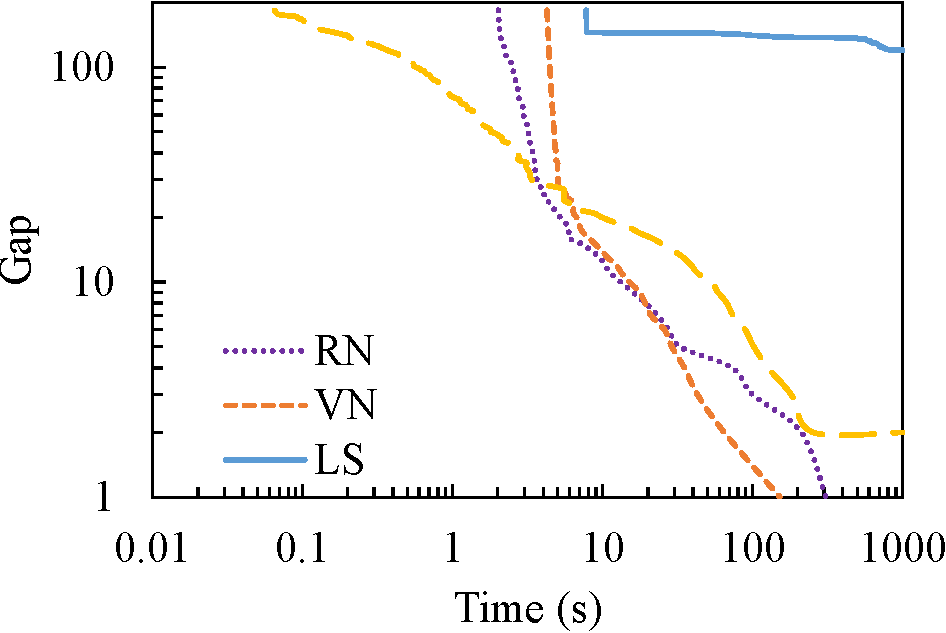
\includegraphics[width=0.5\columnwidth]{fig-SampleFigure.pdf}
	\caption{Evolution of the objective value gaps.}
	\label{fig:columnwidth}
\end{szxfig}

~\\\xoutline{\zw{单页宽图片与子图。}\yw{Single-page figure and sub-figures.}}
\begin{szxfig*}[!tb]
	\centering
	\begin{subfigure}[b]{0.31\textwidth}
		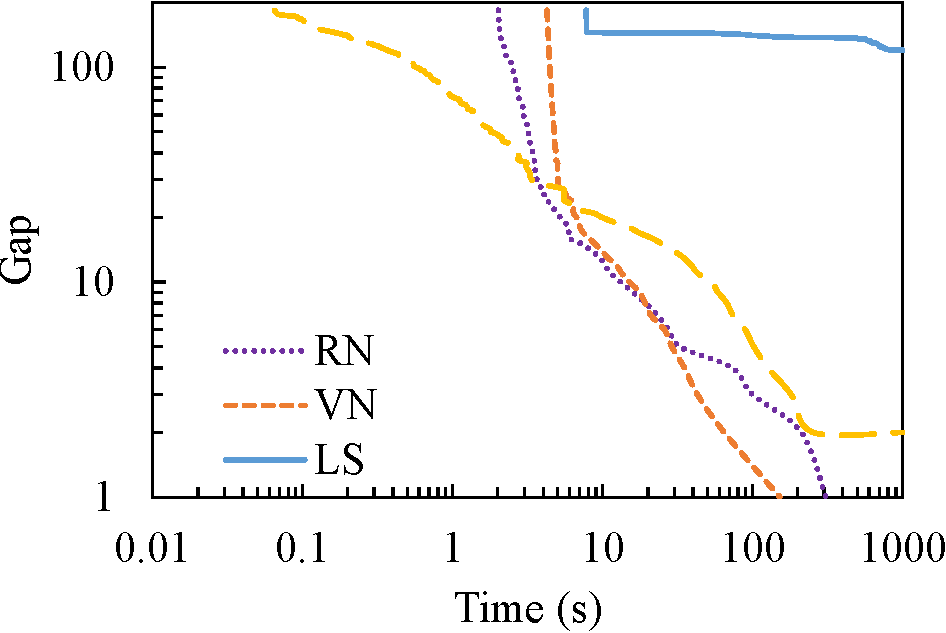
\includegraphics[width=\textwidth]{fig-SampleFigure.pdf}
		\xfigcap{Plot1.}
		\label{fig:convergence1}
	\end{subfigure}
	~
	\begin{subfigure}[b]{0.31\textwidth}
		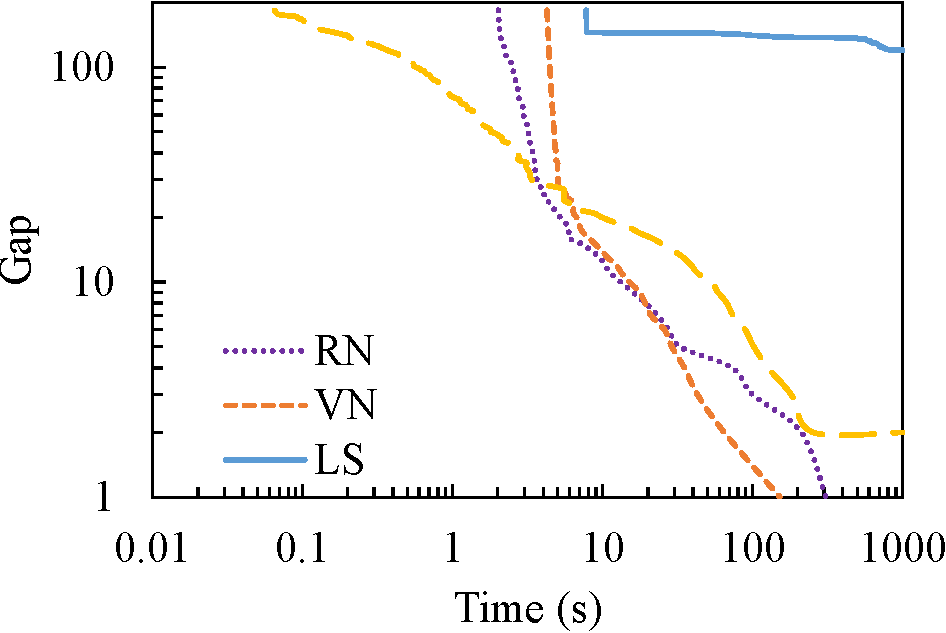
\includegraphics[width=\textwidth]{fig-SampleFigure.pdf}
		\xfigcap{Plot2.}
		\label{fig:convergence2}
	\end{subfigure}
	~
	\begin{subfigure}[b]{0.31\textwidth}
		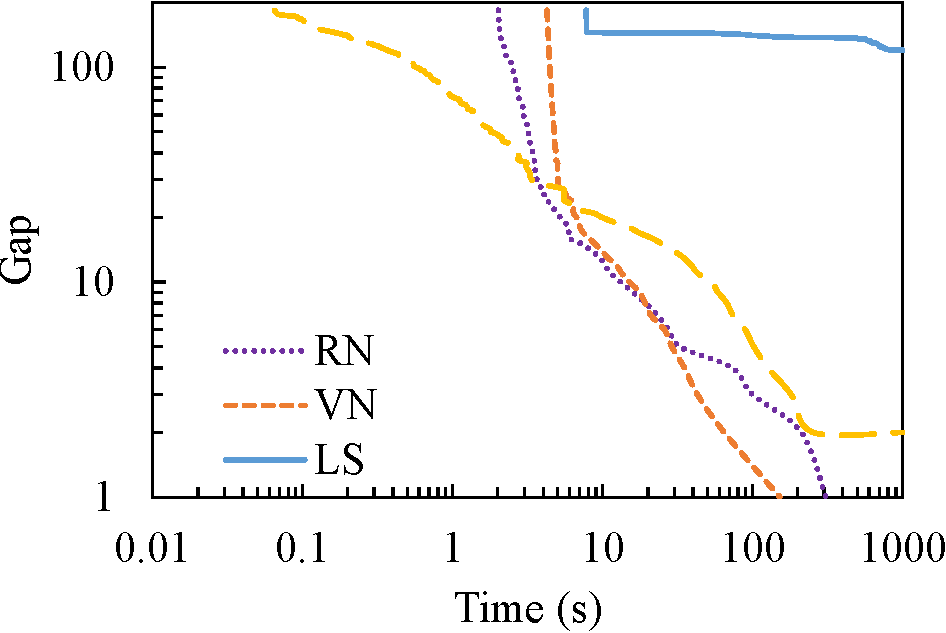
\includegraphics[width=\textwidth]{fig-SampleFigure.pdf}
		\xfigcap{Plot3.}
		\label{fig:convergence3}
	\end{subfigure}
	\xfigcap{Evolution of the objective value gaps again.}
	\label{fig:textwidth}
\end{szxfig*}

~\\\xoutline{\zw{引用图片与子图。}\yw{Refer to figure and sub-figures.}}
\xreffig{fig:columnwidth} illustrates ...
\xreffig{fig:textwidth} demonstrates ...
\xreffig{fig:convergence2} shows ...

~\\\xoutline{\zw{单栏宽表格(单页宽表格与图片类似加“*”即可)。}\yw{Single-column table (for single-page table, just add ``*'' as figure do).}}
\begin{szxtab}[!tb]
	\newcommand{\B}[1]{\textbf{#1}}
%	\setlength{\tabcolsep}{1pt}
	\resizebox{\columnwidth}{!}{%
		\begin{tabular}{lrcrrrr}
			\xtrule
			\multirow{2}{*}{Instance} & \multicolumn{1}{c}{RefAlg} &  &        \multicolumn{4}{c}{\AlgName{}}        \\
			\xcrule{2-2}\xcrule{4-7}  &                      Score &  & Score-1h &  Improve &     Score-2h & Improve \\
			\xmrule
			case3                     &                      11610 &  &    11848 &      238 &    \B{11880} &     270 \\
			case4                     &                    2064790 &  &  2071515 &     6725 &  \B{2076537} &   11747 \\
			\xmrule
			Total                     &                   11178613 &  & 11220796 &    42183 & \B{11246076} &   67463 \\
			Normalized                &                    99.62\% &  &        - & 100.00\% &     100.00\% &         \\
			\xbrule
		\end{tabular}%
	}
	\xtabcap{Comparison with the state-of-the-art algorithms.}
	\label{tab:CmpSOTA}
\end{szxtab}

~\\\xoutline{\zw{引用表格。}\yw{Refer to table.}}
\xrefTab{tab:CmpSOTA} reports ...
\xreftab{tab:CmpSOTA} presents ...

~\\\xoutline{\zw{单栏宽算法(单页宽算法与图片类似加“*”即可)。}\yw{Single-column algorithm (for single-page algorithm, just add ``*'' as figure do).}}
\begin{szxalg}[!tb]
	\caption{\label{alg:framework}General framework of \AlgName{}}
	\KwIn{Graph $\TopoGraph(\VertexSet, \EdgeSet)$}
	\KwOut{The best solution $s^{*}$ found so far}
	$f^{*} \leftarrow +\infty$\;\label{line:init}
	\While{time limit is not met\label{line:term}}
	{
		\If{$f(s) < f^{*}_{iter}$\label{line:check}}
		{
			$f^{*}_{iter} \leftarrow f(s)$\;\label{line:update}
		}
		\Else
		{
			$stagnation \leftarrow stagnation + 1$\;
		}
	}
	return $s^{*}$\;
\end{szxalg}

~\\\xoutline{\zw{引用算法与代码行。}\yw{Refer to algorithm and lines.}}
\xrefalg{alg:framework} gives ...
\xrefline{line:init} ...
\xrefline{line:init,line:update} ...
\xrefline{line:term,line:check,line:update} ...

~\\\xoutline{\zw{源代码。}\yw{Source code.}}
\begin{lstlisting}[language=json,caption={Sample configuration file.},label={code:cfg}]
{
  "random_seed": 42,
  "acceptance_rule": {
    "type": "LAHC",
  },
  "inter_operators": [
    [ "Relocate" ],
    [ "Swap<2, 0>", "Swap<2, 1>", "Swap<2, 2>" ]
  ],
  "intra_operators": [ "Exchange", "OrOpt<1>" ]
}
\end{lstlisting}

~\\\xoutline{\zw{引用源代码。}\yw{Refer to source code.}}
\xrefcode{code:cfg} gives ...

~\\\xoutline{\zw{数学定义。}\yw{Mathematical definition.}}
\begin{definition}
some definition.
\label{def:sample}
\end{definition}

~\\\xoutline{\zw{引用数学定义。}\yw{Refer to mathematical definition.}}
\xrefdef{def:sample} is typeset by \verb`\xrefdef{def:sample}`.

~\\\xoutline{\zw{数学命题及其证明。}\yw{Mathematical proposition.}}
\begin{proposition}
some proposition.
\label{prop:sample}
\end{proposition}
\begin{proof}
some proof.
\qedhere
\end{proof}

~\\\xoutline{\zw{引用数学命题。}\yw{Refer to mathematical proposition.}}
\xrefprop{prop:sample} is typeset by \verb`\xrefprop{prop:sample}`.

~\\\xoutline{\zw{无编号列表。}\yw{List of items without numbering.}}
\begin{szxitem}
	\item\textbf{First}
	The first item ...
	 
	\item\textbf{Second}
	The second item ...
\end{szxitem}

~\\\xoutline{\zw{带编号列表。}\yw{List of items with numbering.}}
\begin{szxenum}
	\item\textbf{First}
	The first enum ...
	
	\item\textbf{Second}
	The second enum ...
\end{szxenum}


\xsubsec{English writing and checklist}
\label{sec:s3}

\begin{szxenum}
	\item
	\zw{单独标点符号右侧加空格,成对标点符号外侧加空格,连续标点符号之间省略空格。}\yw{}
	The spacing rules are easy, e.g., adding space (i.e., ``~'' character) as this sentence, next sentence, etc.

	\item
	\zw{图片标题可以写成一段话简单介绍图片内容。}\yw{}

	\item
	\zw{表格一般文本左对齐,数字右对齐(严格地说应为精度一致沿小数点对齐)。}\yw{}

	\item
	\zw{如果不方便在标题页加脚注的形式标注通讯作者与基金号,可以在致谢部分注明。}\yw{}

	\item
	\zw{编辑(或自动匹配系统)很有可能从参考文献中找审稿人,应确保文献跟本文相关度较高。此处的较高具体指类似问题类似方法,例如启发式算法的论文应尽量避免引用纯粹理论分析而不具体求解的论文。但如果完全是不同的圈子没有影响,例如AI会议论文引用没在AI会议上发过论文的人的文章。}\yw{}
	
	\item
	\zw{缩写检查法避免写废话或循环论证,例如下面的案例可以通过缩写句子识别出来。}\yw{}
	\begin{szxitem}
		\item ... perturbation ... is to ... perturb ...
		\item the influence of ... is high since ... is the key component of ...
	\end{szxitem}
	
	\item
	\zw{避免过于极端、绝对或带感情色彩的词,尤其是评价他人的算法和结果时,例如“精确算法无法求解大规模算例”、“the results of ... are poor”。}\yw{}
\end{szxenum}

\end{document}
